\documentclass{article}
\usepackage[utf8]{inputenc}
\usepackage{minted}

\usepackage{graphicx}

\title{Variations of the Eight Queens Puzzle}
\author{Madhulika Mitra (k12146811) madhu.mitra07@gmail.com \and
Jakob Weber (k01603774) weberjakob@gmx.at \and
David Auinger (k00755686) K00755686@students.jku.at}
\date{\today}

\begin{document}

\maketitle

\begin{abstract} \noindent
    We implemented a program that solves a generalization of the popular eight queens puzzle in Prolog. Our program not only solves the problem for arbitrary rectangular boards, but also implements various other types of pieces. Further, the program can solve problems combining different types of pieces. We show that our implementation solves already solved problems and present solutions for newly posed problems. Since our program can be easily extended to new types of pieces, this offers a starting point for a multitude of new experiments.
\end{abstract}

\section{Introduction}

The eight queens puzzle is a popular problem posed by Max Brezzel in 1848. The first solutions were published by Franz Nauck two years later \cite{CAMPBELL1977397}. Since then various alterations and have been suggested, for example different board sizes and other pieces.

In this work, our goal is to implement an extended and generalized version of the eight queens puzzle in Prolog. We extend the pieces to also allow find solutions for knights, bishops, rooks and amazons (a fairy chess piece combining the moves of a knight and a queen). These different pieces can be mixed up. It is both able to find one solution as well as count all possible solutions. In additions to this we introduce a variable board size that can be specified in the input.

The remainder of this work is organized as follows: In the next section, we describe our approach and implementation of the Prolog program to solve the problem. Section~\ref{sec:usage} describes how to use our program. Examples of our working implementation are presented in Section~\ref{sec:examples}. Section~\ref{sec:conclusion} concludes this work.

\section{Approach and implementation} \label{sec:approach}

The basic approach of the eight queens puzzle is well researched and there are plenty of implementations in Prolog available online. In our work, we solve a more general problem that covers different types of pieces and variable board sizes. An online solution of the base case that we used to define the basic structure of our programm is implemented by Livaudais \cite{8_queens}.

Our program takes six lists as parameters. The first list defines the desired (rectangular) board size (length and width). The other five lists define the type and number of pieces to be placed on the board. The program supports these types of pieces: knight, bishop, rook, queen, amazon. Then our program runs and outputs a solution for the given board size and sets of pieces, or \verb|false| if no solution exists for the given input parameters.

The \verb|main| function is the starting point and defines the input. Then a function \verb|possibleSolution| initializes the pieces with possible locations. The function \verb|correctSolution| checks if this initialization is a correct solution. If \verb|correctSolution| fails, Prolog tracks back and tries with another initilization until a solution is found or the search space is exhausted.
\begin{minted}{prolog}
main([SizeX, SizeY], NS, BS, RS, QS, AS) :-
	/* first set up the board locations in Loc */
	findall([X, Y], (between(1, SizeX, X), between(1, SizeY, Y)), Loc),
	/* then find a possible solution */
	possibleSolution(Loc, NS, BS, RS, QS, AS),
	/* finally check if solution is correct */
	correctSolution(Loc, NS, BS, RS, QS, AS).
\end{minted}

The function \verb|correctSolution| calls a function for each type of piece that checks if the pieces (\emph{e.g.} knights) attack each other or any other piece on the board.
\begin{minted}{prolog}
checkKnights(Loc, NS, PS_N),
\end{minted}
\begin{itemize}
    \item Loc is a list of all board locations (e.g. for a 2x2 board this would be [[1,1],[1,2],[2,1],[2,2]])
    \item NS is the list of Knights
    \item PS\_N is the list of all pieces except of Knights
\end{itemize}

Allowing different types of pieces incurs some particular challenges. We will first discuss these challenges before going to the types of pieces in detail.

\subsection{Challenges}

When there is just one type of piece, showing that a specific piece does not attack any other piece suffices to know that this piece is not attacked by any other piece (a queen is not attacked by another queen unless itself attacks the other queen). With different types of pieces, this assumption is no longer valid. For example, a queen that is not attacking a knight might still be attacked by the same knight. This is important to understand for our approach since most solutions for the eight queens puzzle make use of this assumption by only checking that a newly placed queen is not attacking any other queen, but not going the other way round. Therefore, in order to solve the problem in a more general way for different types of pieces, we can only make use of this assumption within the same type of piece, but for other types we need to check against all other pieces. To illustrate this, take for example a problem with two bishops and two queens. In order to verify that a solution is correct, one bishops has to be checked against the other bishop and the queens, the second bishop against the queens only, one queen again against both bishops and the other queen, the second queen against both bishops. This shows that with a higher number of types checking the correctness of a solution becomes increasingly computationally costly.

Another challenge that was arising was caused by the fact that Prolog handles lists as ordered lists and has no meaning for unordered sets. This is particularly unfortunate for this problem as we do not want to consider permutations as unique solutions. However, in a permutation of an ordered lists creates a different list, such that Prolog considers a permutation a unique solution. In order to exclude permutations from the solutions, we defined an order of the locations on the board and required that pieces of the same type must be placed in strictly increasing locations.

\subsection{Pieces in detail}

There are essentially two possibilities how a piece can attack: by moving to defined locations relative to the current location (like the knight) or by moving an arbitrary distance in a certain direction (like the bishop, rook and queen). The amazon is a mixture of both. By understanding this, we are able to implement functions that check if a piece attacks another piece.

The knight can be solved with a function that checks if no other piece is in the same location or any of the eight locations possibly attacked by the knight. For a given knight and a list of other pieces, this function makes use of the Prolog feature of splitting lists, checking the knight against the first element from the list of other pieces, than recursively calling the function with the rest of the list until the list of other pieces is empty. By recursively checking all knights in this way, we have solved the problem for the knight.

To solve the bishop we implemented a function that checks if another piece is in the same major diagonal or the same minor diagonal of the bishop. This is done recursively for all other pieces similarly to the knight as already described. In a similar way, the rook is solved by checking the row and column of the location of the rook. The queen essentially combines the check of the bishop and the rook. Finally, we implemented a function that checks the amazon be using the same checks as for the knight and the queen.

\section{Usage} \label{sec:usage}
\subsection{Input}
The main function takes the board size [SizeX, SizeY] and a list for each of the pieces:
\begin{minted}{prolog}
main([SizeX, SizeY], NS, BS, RS, QS, AS)
\end{minted}
the input for the 8 Queen problem would for example look like:
\begin{minted}{prolog}
?- main([8, 8], [], [], [], [Q1, Q2, Q3, Q4, Q5, Q6, Q7, Q8], []).
\end{minted}
it is possible to combine different pieces too:
\begin{minted}{prolog}
?- main([5,5],[N],[B],[R],[Q],[A]).
\end{minted}

\subsection{Output}
The Output shows a possible solution of the problem:
\begin{minted}{prolog}
?- main([5,5],[N],[B],[R],[Q],[A]).
N = [1, 2],
B = [1, 3],
R = [2, 5],
Q = [4, 1],
A = [5, 4] .
\end{minted}
With ";" the next solution is searched.

With the same input variables the function \verb|countSolutions| prints the number of solutions of the input problem:
\begin{minted}{prolog}
?- countSolutions([8, 8], [], [], [], [Q1, Q2, Q3, Q4, Q5, Q6, Q7, Q8], []).
92
true.
\end{minted}

\section{Examples} \label{sec:examples}

We test our implementation on different problems. At first we verify the correctness on the well-known eight queens problem. When we run the program with this input, we obtain as first solution:
\begin{minted}{prolog}
?- main([8, 8], [], [], [], [Q1, Q2, Q3, Q4, Q5, Q6, Q7, Q8], []).
Q1 = [1, 4],
Q2 = [2, 2],
Q3 = [3, 7],
Q4 = [4, 3],
Q5 = [5, 6],
Q6 = [6, 8],
Q7 = [7, 5],
Q8 = [8, 1] .
\end{minted}

\begin{figure}[h]
\centering
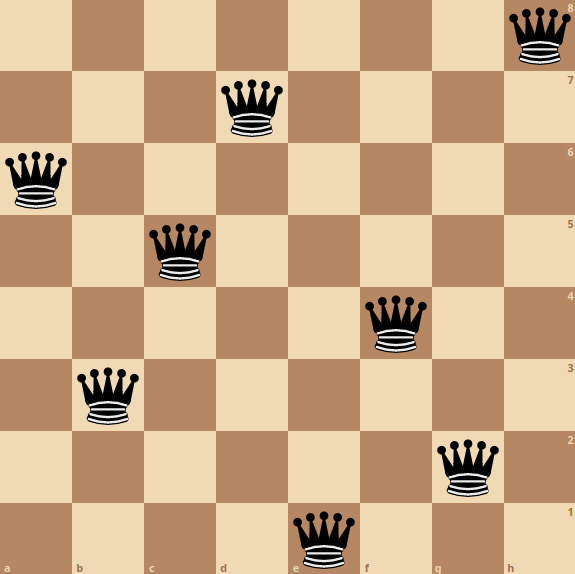
\includegraphics[width=\linewidth/2]{8queens.png}
\caption{A correct solution of the eight queens puzzle}
\label{fig:8_queens}
\end{figure}

Figure~\ref{fig:8_queens} depicts this solution. It can easily be verified that this indeed is a correct solution.

Next, we present an example for mixed types of pieces. The following command finds solutions for each of the five types of pieces once on a 5x5 board:
\begin{minted}{prolog}
?- main([5,5],[N],[B],[R],[Q],[A]).
N = [1, 2],
B = [1, 3],
R = [2, 5],
Q = [4, 1],
A = [5, 4] .
\end{minted}

\begin{figure}[h]
\centering
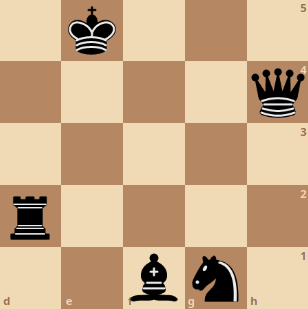
\includegraphics[width=\linewidth/2]{prolog_mixed_solution.png}
\caption{A solution for a problem with mixed types of pieces}
\label{fig:mixed_solution}
\end{figure}

This solution is shown in Figure~\ref{fig:mixed_solution}. We can also count the number of solutions:
\begin{minted}{prolog}
?- countSolutions([5,5],[N],[B],[R],[Q],[A]).
96
\end{minted}

\section{Conclusion} \label{sec:conclusion}

We have implemented a Prolog program that solves a generalization of the eight queens puzzle. We have shown that our program is able not only to solve the classic eight queens puzzle, but also solve similar problems on other rectangular board sizes with different types of pieces. Most interestingly, our program is able to handle combinations and mixtures of different types of pieces.

For future work, this program can be easily extended to other types of pieces, such that a multitude of new problems can be posed and solved. It might also be of interest to search for explicit solutions for different problems with different pieces as has been done for the $n$ queens problem \cite{Bernhardsson1991ExplicitST}.

\bibliographystyle{abbrv}
\bibliography{bibliography}

\section*{Appendix Code}

\begin{minted}{prolog}

/* usage: The main function takes 6 lists as parameters. The first list
 *        contains two elements, the length and with of the board (e.g. [8, 8]
 *        for a standard 8x8 chess board. The remaining 5 lists contain the
 *        pieces to be places on the board in this order: knights, bishops,
 *        rooks, queens, amazons.
 *
 * example: classic 8 queens problem
 *          main([8, 8], [], [], [], [Q1, Q2, Q3, Q4, Q5, Q6, Q7, Q8], []). */

main([SizeX, SizeY], NS, BS, RS, QS, AS) :-
	/* first set up the board locations in Loc */
	findall([X, Y], (between(1, SizeX, X), between(1, SizeY, Y)), Loc),
	/* then find a possible solution */
	possibleSolution(Loc, NS, BS, RS, QS, AS),
	/* finally check if solution is correct */
	correctSolution(Loc, NS, BS, RS, QS, AS).

/* Instead of getting one solution, we can also ask to count all possible solutions with countSolutions().
*/
countSolutions([SizeX, SizeY], NS, BS, RS, QS, AS) :-
	findall(.,main([SizeX, SizeY], NS, BS, RS, QS, AS), Ls),
	length(Ls,L),
	write(L).

/* Initializes the pieces with possible values. The result is not necessarily a
 * correct solution. */
possibleSolution(Loc, NS, BS, RS, QS, AS) :-
	checkKnights(Loc, NS, []),
	checkBishops(Loc, BS, []),
	checkRooks(Loc, RS, []),
	checkQueens(Loc, QS, []),
	checkAmazons(Loc, AS, []).

/* Checks if the values are a correct solution for the problem. */
correctSolution(Loc, NS, BS, RS, QS, AS) :-
	append([AS, RS, BS, QS], PS_N),
	checkKnights(Loc, NS, PS_N),
	append([AS, NS, RS, QS], PS_B),
	checkBishops(Loc, BS, PS_B),
	append([AS, NS, BS, QS], PS_R),
	checkRooks(Loc, RS, PS_R),
	append([AS, NS, RS, BS], PS_Q),
	checkQueens(Loc, QS, PS_Q),
	append([NS, RS, BS, QS], PS_A),
	checkAmazons(Loc, AS, PS_A).

/* The function validOrder is a helper function to ensure we exlude
 * permutations, i.e. solutions that only differ in the order of pieces of the
 * same type. */

/* base case */
validOrder(_, [_|_], []).

validOrder(Loc, [A|B], [[C|D]|PS]) :-
	/* make sure this piece is in a location strictly less than the next */
	(A < C -> true; (A == C, B < D)),
	/* recursive call */
	validOrder(Loc, [A|B], PS).

/* Following are various checkXXX functions that check for each type of piece
 * if all pieces of this type do not attack any other piece. Each of these
 * functions takes 3 lists as parameters in the form
 *     checkXXX(Loc, XXXPieces, OtherPieces)
 * where
 *     Loc - is the list of board locations
 *     XXXPieces - is the list of pieces of this type
 *     OtherPieces - is the list of all pieces of all other types
 *
 * This function is evaluated recursively, starting from the end of the list of
 * pieces of this type (XXXPieces). The base case (XXXPieces is the empty list)
 * is always true. For the recursive call we split the list XXXPieces into the
 * first piece and the list of remaining pieces. Then we do the recursive call
 * with the list of remaining pieces. When the recursion succeeds, we require
 * that the first piece must be on a location of the board. Finally, we check
 * that the first piece does not attack any piece of the list of remaining
 * pieces (XXXPieces minus the first piece) or the list of other pieces
 * (OtherPieces) combined.
 *
 * To check this, we have a function validXXX for each type of piece. In
 * contrast to the checkXXX function (which is basically a duplication for each
 * type of piece), the validXXX function is specific for each type of piece:
 * this function is aware of the directions a piece can attack other pieces.
 * This function takes 3 lists as parameters in the form
 *     validXXX(Loc, XXXPiece, OtherPieces)
 * where
 *     Loc - is the list of board locations
 *     XXXPiece - is the list for the location of this piece in the form [x, y]
 *     OtherPieces - is the list of all other pieces
 *
 * The validXXX function again is evaluated recursively. The base (OtherPieces)
 * is the empty list) is always true. For the recursive call we split the list
 * OtherPieces into the first piece and the list of remaining pieces. We then
 * require that this piece (XXXPiece) does not attack the first piece of
 * OtherPieces. When this succeeds, we recursively call the function with the
 * list of remaining pieces.
 */

/* base case */
checkKnights(_, [], _).

checkKnights(Loc, [N|NS], PS) :-
	/* recursive call */
	checkKnights(Loc, NS, PS),
	/* make sure first knight is on board */
	member(N, Loc),
	/* exclude permutations */
	validOrder(Loc, N, NS),
	/* make sure first knight does not attack any other piece */
	append(NS, PS, NPS),
	validKnights(Loc, N, NPS).

/* base case */
validKnights(_, [_|_], []).

validKnights(Loc, [A|B], [[C|D]|PS]) :-
	/* make sure [A|B] and [C|D] are not in the same location */
	(A =\= C -> true; B =\= D),
	/* make sure [A|B] does not reach [C|D] with a knight's move */
	(A+2 =\= C -> true; B+1 =\= D),
	(A+2 =\= C -> true; B-1 =\= D),
	(A-2 =\= C -> true; B+1 =\= D),
	(A-2 =\= C -> true; B-1 =\= D),
	(A+1 =\= C -> true; B+2 =\= D),
	(A+1 =\= C -> true; B-2 =\= D),
	(A-1 =\= C -> true; B+2 =\= D),
	(A-1 =\= C -> true; B-2 =\= D),
	/* recursive call */
	validKnights(Loc, [A|B], PS).

/* base case */
checkBishops(_, [], _).

checkBishops(Loc, [B|BS], PS) :-
	/* recursive call */
	checkBishops(Loc, BS, PS),
	/* make sure first bishop is on board */
	member(B, Loc),
	/* exclude permutations */
	validOrder(Loc, B, BS),
	/* make sure first bishop does not attack any other piece */
	append(BS, PS, BPS),
	validBishops(B, BPS).

/* base case */
validBishops([_|_], []).

validBishops([A|B], [[C|D]|PS]) :-
	/* make sure they are not in the same major diagonal */
	C - A =\= D - B,
	/* make sure they are not in the same minor diagonal */
	C - A =\= B - D,
	/* recursive call */
	validBishops([A|B], PS).

/* base case */
checkRooks(_, [], _).

checkRooks(Loc, [R|RS], PS) :-
	/* recursive call */
	checkRooks(Loc, RS, PS),
	/* make sure first rook is on board */
	member(R, Loc),
	/* exclude permutations */
	validOrder(Loc, R, RS),
	/* make sure first rook does not attack any other piece */
	append(RS, PS, RPS),
	validRooks(R, RPS).

/* base case */
validRooks([_|_], []).

validRooks([A|B], [[C|D]|PS]) :-
	/* make sure they are not in the same row */
	A =\= C,
	/* make sure they are not in the same column */
	B =\= D,
	/* recursive call */
	validRooks([A|B], PS).

/* base case */
checkQueens(_, [], _).

checkQueens(Loc, [Q|QS], PS) :-
	/* recursive call */
	checkQueens(Loc, QS, PS),
	/* make sure first queen is on board */
	member(Q, Loc),
	/* exclude permutations */
	validOrder(Loc, Q, QS),
	/* make sure first queen does not attack any other piece */
	append(QS, PS, QPS),
	validQueens(Q, QPS).

/* base case */
validQueens([_|_], []).

validQueens([A|B], [[C|D]|PS]) :-
	/* make sure they are not in the same row */
	A =\= C,
	/* make sure they are not in the same column */
	B =\= D,
	/* make sure they are not in the same major diagonal */
	C - A =\= D - B,
	/* make sure they are not in the same minor diagonal */
	C - A =\= B - D,
	/* recursive call */
	validQueens([A|B], PS).

/* base case */
checkAmazons(_, [], _).

checkAmazons(Loc, [A|AS], PS) :-
	/* recursive call */
	checkAmazons(Loc, AS, PS),
	/* make sure first amazon is on board */
	member(A, Loc),
	/* exclude permutations */
	validOrder(Loc, A, AS),
	/* make sure first amazon does not attack any other piece */
	append(AS, PS, APS),
	validAmazons(Loc, A, APS).

/* base case */
validAmazons(_, [_|_], []).

validAmazons(Loc, [A|B], [[C|D]|PS]) :-
	/* make sure they are not in the same row */
	A =\= C,
	/* make sure they are not in the same column */
	B =\= D,
	/* make sure they are not in the same major diagonal */
	C - A =\= D - B,
	/* make sure they are not in the same minor diagonal */
	C - A =\= B - D,
	/* make sure [A|B] does not reach [C|D] with a knight's move */
	(A+2 =\= C -> true; B+1 =\= D),
	(A+2 =\= C -> true; B-1 =\= D),
	(A-2 =\= C -> true; B+1 =\= D),
	(A-2 =\= C -> true; B-1 =\= D),
	(A+1 =\= C -> true; B+2 =\= D),
	(A+1 =\= C -> true; B-2 =\= D),
	(A-1 =\= C -> true; B+2 =\= D),
	(A-1 =\= C -> true; B-2 =\= D),
	/* recursive call */
	validAmazons(Loc, [A|B], PS).
\end{minted}

\end{document}
